\section{Exercises: basic constructions}
\label{section-exercises-constructions}

\begin{exercise}
\label{exercise-trace-is-independent-of-coordinates}
Show that the trace is independent of coordinates.
\end{exercise}

\begin{proof}[Solution]
Let $A$ be an endomorphism of a vector space. By definition
$$
\text{tr}A=A_i^i
$$
Now if $P$ is any invertible matrix,
$$
\text{tr}PAP^{-1}=P^j_iA_j^k\overline{P}_k^i=P^j_i\overline{P}_k^iA_j^k
=\delta_k^jA_j^k=A_j^j
$$
where $\overline{P}$ denotes the indices of the inverse of $P$.
\end{proof}

The following two lemmas are preparatory results for Exercise
\ref{exercise-derivative-of-determinant}.

\begin{lemma}
\label{lemma-for-derivative-of-determinant1}
Let $\gamma_1,...,\gamma_m:(a,b)\to\mathbb{R}^n$ be smooth curves and define 
$f:(a,b)\to\mathbb{R}$ by $f(t)=\det(\gamma_1(t),\ldots,\gamma_n(t))$. Then
$$
f'(t_0)
=\sum_{k=1}^{m}\det(\gamma_1(t_0),\ldots,\gamma'_k(t_0),\ldots,\gamma_m(t_0)).
$$
\end{lemma}

\begin{proof}
This follows from multilinearity of the determinant using the definition of
derivative of a map $g:\mathbb{R}^n \to \mathbb{R}^m$ as given by
$$
g(x+h)-g(x)=L(x)h+\varepsilon(x;h)
$$
where $\varepsilon$ is $o(h)$, meaning that  $\lim_{h \to 0}
\frac{\varepsilon(x;h)}{h}=0$.

More exactly, since $\gamma_k$ are smooth we may write
$$
\gamma(t_0+h)=\gamma_k(t_0)+h\gamma'_k(t_0)+\varepsilon_k(h)
$$
We substitute into the determinant…
\end{proof}

\begin{lemma}
\label{lemma-for-derivative-of-determinant2}
Let $M \in \text{Mat}_{n\times n}(\mathbb{R})$ be any matrix. Let 
$f:\mathbb{T}\to \mathbb{R}$ be defined by $f(t):=\det(\text{Id}+tM)$. Then 
$f'(0)=\text{tr}(M)$.
\end{lemma}

\begin{proof}
This follows easily from Lemma \ref{lemma-for-derivative-of-determinant1}.
\end{proof}

\begin{exercise}
\label{exercise-derivative-of-determinant}
Let $A(t)$ be a one parameter family of matrices. Compute $\det A(t)'$.
\end{exercise}

\begin{proof}[Physicist's solution]
The determinant of a matrix is given by the product of its eigenvalues
$\lambda_i$. Taking logarithms we see that
$$
\text{log}\det A(t)=\text{log}\prod_{i}\lambda_i=\sum_{i}\text{log}\lambda_i
$$
and differentiating we obtain
$$
\frac{\det A(t)'}{\det A(t)}=\sum_i \frac{\lambda_i'}{\lambda_i}
=\text{tr} A'(t)A(t)^{-1}.
$$
with the caveat that we must confirm whether the functions $\lambda_i$ are
differentiable. (Still pending…)
\end{proof}

\begin{proof}[Solution]
Consider the determinant as a function 
$\det:\text{GL}(n,\mathbb{R})\to\mathbb{R}$. Is total derivative at 
$A \in \text{GL}(n,\mathbb{R})$ is a linear map 
$\text{GL}(n,\mathbb{R})\to \mathbb{R}$ which when evaluated at a matrix
$H\in\text{GL}(n\mathbb{R})$ is defined by
$$
\det(A)'H=\lim_{t\to0}\frac{\det(A+tH)-\det(A)}{t} 
$$
Now define $f(t):=\det(A+tH)$ so that the latter equation reads $f'(0)$. Then
observe that
$$
f(t)=\det(A+tH)=\det(A(\text{Id}+tA^{-1}H)=\det(A)\det(\text{Id}+tA^{-1}H).
$$
By Lemma \ref{lemma-for-derivative-of-determinant2} we conclude that 
$f(t)=\det(A)\text{tr}(A^{-1}H)$. Letting $H=A(t)'$ we obtain the result since
by the chain rule $\det(A(t))'=\det(A(t))'A(t)'$.
\end{proof}

\begin{exercise}
\label{exercise-Levi-Civita-connection-of-product}
Let $P$ and $Q$ be Riemannian manidols. Sow that the Levi-Civita connection of
the product metric is given by
$\nabla_{Y_1+Y_2}(X_1+X_2)=\nabla^P_{Y_1}X_1+\nabla^Q_{Y_2}X_2$.
\end{exercise}

\begin{exercise}
\label{exercise-totally-geodesic-submanifolds-of-product}
Let $P$ and $Q$ be Riemannian manifolds. Show that for any $p \in P$ and $q \in
Q$, $P\times \{q\}$ and $\{q\}\times P$ are totally geodesic
submanifolds of $P \times Q$.
\end{exercise}

\begin{proof}[Solution]
Let $v \in T_{(p,q)}(P\times\{q_0\})$ and consider the geodesic
 $\text{exp}_p^{P\times Q}(tv)$. Then
its acceleration vanishes since the Levi-Civita connection of the product metric
is given by Exercise \ref{exercise-Levi-Civita-connection-of-product}, and the
component along $Q$ vanishes.
\end{proof}

The following exercise is important for future constructions identifying Jacobi
fields, Hessian operators and mean curvature of geodesic spheres.

\begin{exercise}
\label{exercise-mean-curvature}
Lista 4, Exercício 8. Let $(M,g)$ be a Riemannian manifold. Suppose that there
is a function $f \in C^\infty(M)$ such that $0 \in \mathbb{R}$ is a regular
value of $f$ and let $\Sigma:=f^{-1}(0)$.
\begin{enumerate}
\item Let $N=\frac{\nabla f}{|\nabla f| \in \mathfrak{X}^\perp(\Sigma)}$. Mostre
que
$$
\left<\alpha_{\Sigma}(X,Y),N\right>=-\frac{\text{Hess}(f)(X,Y)}{|\nabla f|},
$$
para todos $X,Y \in \mathfrak{X}(\Sigma)$.

\item Show that the mean curvature of $\Sigma$ is given by
$$
H_{\Sigma}=-\frac{1}{n}\mathsf{div}\left(\frac{\nabla f}{|\nabla f|}\right)
$$
\end{enumerate}
{\it Note.} The notation in item (1) identifies fields using the differential of
the inclusion map, as is customary.
\end{exercise}

\begin{proof}
\begin{enumerate}
\item One one hand,
 $$
\left<\alpha(X,Y),\nabla f\right>=-\left<Y,A_{\nabla f}X\right>
$$
by Remark \ref{remark-second-fundamental-form-and-shape-operator-are-adjoint}.
On the other hand,
$$
\text{Hess}(f)(X,Y)=\left<\tilde{\nabla}_X \nabla f,Y\right>=
\left<-A_{\nabla f}X+\nabla_X^\perp \nabla f,Y\right>,
$$
then multiply by $\frac{1}{|\nabla f|}$.

\item To compute the divergence as the trace of the gradient we need an
orthonormal frame of $M$. So let $E_i$ be an orthonormal frame of $\Sigma$ and
add $\frac{\nabla f}{|\nabla f|}$ to obtain a frame of $M$. Then:
\begin{align*}
\text{div}\left(\frac{\nabla f}{|\nabla f|}\right)&=\sum
\left<\tilde{\nabla}_{E_i}\frac{\nabla f}{|\nabla
f|},E_i\right>+\underbrace{\left<\tilde{\nabla f}_{\frac{\nabla f}{|\nabla
f|}}\frac{\nabla f}{|\nabla f|},\frac{\nabla f}{|\nabla
f|}\right>}_{\frac{1}{2}\left|\frac{\nabla f}{|\nabla f|}\right|^2=0}\\
&=\sum \left<-A_{\frac{\nabla f}{|\nabla f|}}E_i,E_i\right>\\
&=-\text{tr}(X \mapsto A_{\frac{\nabla f}{|\nabla f|}}X=-nH_{\Sigma}(p)
\end{align*}

\end{enumerate}
\end{proof}

\begin{exercise}
\label{exercise-curvatures-in-product}
Lista 5, Exercise 1. Let $(M_1,g_1)$ and $(M_2,g_2)$ be Riemannian manifolds and
let $M_1\times M_2$ be equipped with the product metric $g:=g_1\oplus g_2$. Show
that the curvature tensor, the Ricci curvature and the scalar curvature of $g$
are given by
\begin{enumerate}
\item $R=\pi_1^*R_1+\pi_2^*\mathbb{R}^2$,
\item $\text{Ric}=\pi_1^*\text{Ric}_1+\pi_2^*\text{Ric}_2$,
\item $\text{scal}=\pi_1^*\text{scal}_1+\pi_2^*\text{scal}_2$
\end{enumerate}
where $\pi_i:M_1\times M_2\to M_i$ are the projections.
\end{exercise}

\begin{exercise}
\label{exercise-fixed-point-set-of-isometry-is-totally-geodesic-submanifold}
\cite{pet}, Proposition 5.6.5. Let $f:M\to M$ be an isometry. Show that the
connected component of the fixed points of $f$ is a totally geodesic
submanifold.
\end{exercise}

\begin{proof}
The trick is to show that the eigenvectors of $df$ are in bijection with the
fixed point set of $f$. For this consider an eigenvector, a geodesic realising 
the vector, map it with $f$ and notice it must coincide with the original 
geodesic because $f$ is an isometry and the point is a fixed point. This shows
that the fixed point set is a submanifold since it is parametrized as a linear
subspace under geodesic coordinate charts. It also shows that the fixes point
set is totally geodesic.
\end{proof}
\section{Exercises: global differential geometry}
\label{section-exercises-global-differential-geometry}

\begin{exercise}
\label{exercise-geodesica-sem-pontos-conjugados-e-localmente-minimizante}
$\gamma$ geodésica sem pontos conjugados em $[0,a]$. Então $\gamma$ é localmente
minimizante.
\end{exercise}

\begin{proof}
Temos dois casos:
\begin{enumerate}
\item Se $E''(0)<0$ usamos o teorema do índice. Isto é, não é possível que
 $E''(0)<0$ porque isso implica que o índice da forma do índice é diferente
 de zero, ou seja, existem pontos conjugados.
\item Se $E''(0)=0$,
\begin{enumerate}
\item[(0)] Como $\gamma$ não tem pontos conjugados, então $I$ não tem
nulidade em todo  $\mathcal{V}$.
\item $I_{\mathcal{V}^-}$ não tem índice nem nulidade. Segue do ponto anterior + 
algum passo na prova.
\item $I_{\mathcal{V}^-}$ não tem índice.
\item 2+3 dão que $I_{\mathcal{V}^-}>0$.
\item Logo $I>0$.
\end{enumerate}
\end{enumerate}
\end{proof}

\begin{exercise}[Warped product]
\label{exercise-wraped-product}
Para $(M,g_M)$ e $(N,g_N)$ e $f:M \to \mathbb{R}_+$, definimos o {\it warped
product} como sendo o produto cartesiano $M\times N$ com a métrica 
 $g_M+f^2g_N$.

Mostre que se os fatores são completos, o warped product é completo.
\end{exercise}

\begin{exercise}
\label{exercise-two-submanifolds}
\cite{doc} Chapter IX, Exercise 5. Sejam $N_1$ e $N_2$ duas subvariedades
 fechadas e disjuntas de uma variedade Riemanniana compacta.
\begin{enumerate}
\item Mostre que a distância entre $N_1$ e $N_2$ é realizada por uma geodésica
	$\gamma$ perpendicular a ambas $N_1$ e $N_2$.
\item Mostre que, para qualquer variação ortogonal $h(t,s)$ de $\gamma$, com
$h(0,s) \in N_1$ e $h(\ell,s) \in N_2$, tem-se para a fórmula da segunda
variação a seguinte expressão
$$
\frac{1}{2}E''(0)=I_{\ell}(V,V)+
\left<V(\ell),A_{\gamma'(\ell)}^{(2)}V(\ell)\right>
-\left<V(0),A^{(1)}_{\gamma'(0)}(V(0))\right>
$$
\end{enumerate}
\end{exercise}

\begin{proof}[Solution]
\begin{enumerate}
\item Since both submanifolds are compact, there exists a minimizing geodesic
$\gamma$ joining them. Then we can apply the first variation formula. Consider a
variation that fixes $\gamma$ everywhere but in a small neighbourhood of one of
the contact points. We realise by Eq. \ref{equation-first-variation-formula}
that it must be orthogonal. A similar procedure proves the other endpoint also
arrives orthogonally.

\item By the previous item, we
know that $\gamma'$ is orthogonal to the curves $h(0,s)$ and $h(\ell,s)$. Then
we can differentiate using the formula for normal sections at the endpoints of
$\gamma$:
$$
\tilde{\nabla}_{V}\gamma'=A^{(i)}_{\gamma'}V+\nabla^{\perp,i}_V\gamma'
$$
When computing $V\left<\gamma',\gamma'\right>$ we obtain
$\left<\nabla^{\perp,i}_V\gamma',\gamma'\right>=0$ since the shape operator is
tangent to the submanifolds. If $M_1$ and $M_2$ are hypersurfaces we conclude 
that the normal vector $\nabla^{\perp,i}_V\gamma'$ vanishes since it must be a 
multiple of $\gamma'$. Otherwise I'm not sure why this term would vanish.

Now, other than the Index form, in the Second Variation Formula
\ref{equation-second-variation-formula} we have
$\left<\nabla_{\partial_s}V,\gamma'\right>$. Notice that
$$
\left<f_s,f_t\right>_s=\left<f_{ss},f_t\right>+\left<f_s,f_{st}\right>
$$
The left-hand-side will vanish because the variation is orthogonal, giving the
equality we want (modulo a sign) since $f_{st}$ is precisely
$\tilde{\nabla}_V\gamma'$ by the Symmetry Lemma.
\end{enumerate}
\end{proof}

\begin{exercise}
\label{exercise-intersecting-minimal-hypersurfaces}
Let $(M^n,g)$ be a complete Riemannian manifold with $\operatorname{Ric}_M>0$. 
Suppose $M_1$, $M_2$ are minimal (compact?) complete hypersurfaces. Show that 
$M_1 \cap M_2 \neq \emptyset$.
\end{exercise}

\begin{proof}

Let $\gamma$ be a minimizing geodesic joining $p \in M_1$ to $q\in M_2$ and
minimizing the distance between $M_1$ and $M_2$. Let $e_1,\ldots,e_{n-1}\in
T_pM$ be such that along with $\gamma'(0)$ form an orthonormal basis of $T_pM$.
Let $E_i$ be the parallel transport of $e_i$ along $\gamma$. Notice that
$E_i(\ell)$ is tangent to $M_2$ since it is orthogonal to $\gamma'(\ell)$ and
$M_2$ is a hypersurface, but it is not immediate that the variational curve will
be contained in $M_2$ if we define the variation using the exponential map. This
is essential for the second variational formula to vanish since $\gamma$ is
minimizing among curves joining $M_1$ and $M_2$.

We need to produce the variation not from the vector field but from the
variational curves. Take rectifying coordinates for $M_1$ at $p$. Define the
curve $c^i$ as the $i$-th coordinate curve on the whole neighbourhood of $p$
along $\gamma$.

Now take the velocity of $c^i$ for some $t>0$. Parallel transport this vector
along $\gamma$ until it reaches a rectifying neighbourhood of $q$. Along the
path of $\gamma$ we can use the exponential to define a variation. Once in the
rectifying neighbourhood of $q$, we must define by hand the variational curves
to ensure that the curve at $q$ is contained in $M_2$.

Suppose that $\gamma(t_0)$ is in the rectifying neighbourhood of $q$. Consider a
smooth function $\varphi:[t_0,\ell]\to \mathbb{R}$ that is zero at $t_0$ and $1$
at $\ell$. We can smoothly deform the exponential curves to a curve contained in
$M_2$ at $t=\ell$ by defining 
$$
c^s_i(t):=(1-\varphi)\text{exp}_{\gamma(t)}sE_i(t)+\varphi sE_i(t)
$$ 
Notice that the variational vector is orthogonal to $M_2$ at $q$, so that we may
apply Exercise \ref{exercise-two-submanifolds}. Thus we can express the second
variation formula in such a way that when summing over all indices we obtain the
mean curvatures of each submanifold, which vanish, thus obtaining a
contradiction with the hypothesis that $\text{Ric}>0$.
\end{proof}

\begin{exercise}
\label{exercise-even-dimension-positive-K-compact-is-simply-connected}
Prove que $M^{2n},K_M>0$ compacta, então ela é simplesmente conexa.
\end{exercise}

\begin{exercise}
\label{exercise-odd-dimension-positive-K-is-orientable}
$M^{2n+1}$, $K_M>0$ compacta $\implies$ orientável.
\end{exercise}

\begin{proof}
I want to show that $M^{2n+1}$ is diffeomorphic to its double orientable cover
 $\tilde{M}$. Since $M$ is odd-dimensional, so is $\tilde{M}$. 
\end{proof}

O exercício anterior usa Exercício 6 da lista 6. Ou, equivalentemente,

\begin{exercise}
\label{exercise-inverts-orientation-shortened}
Se $M^{2n+1}$ tem $K_M >0$ e $\gamma:S^1 \to M$ inverta orientação, então é
possível encurtar $\gamma$ na sua classe de homotopia.
\end{exercise}

\begin{exercise}
\label{exercise-product-of-compact-does-not-admit-negative-curvature}
Let $N,M$ be compact. Then $N \times M$ does not admit a metric with $K<0$.
\end{exercise}

\begin{proof}
If both $N$ and $M$ are simply connected then they cannot be compact by
Hadamard's theorem. Assume first that both are not simply connected. Then each
has a nontrivial homotopy class, and such a pair generates an abelian subgroup
of $\pi_1(M \times N)$ that is not isomorphic to $\mathbb{Z}$, a contradiction
with Preissman Theorem \ref{theorem-Preissman}.

Now suppose that $N$ is simply connected and $M$ is not. The universal cover of
$M\times N$, if it admits a metric with negative sectional curvature, 
must be a Hadamard manifold, so that $\tilde{M} \times N \cong \mathbb{R}^n$.
Then the induced map on cohomology is injective map ({\bf why?})
$\pi^* :H^{k}(M)\to H^{k}(\tilde{M} \times N)=H^{k}(\mathbb{R}^n)=0$. This means
by Poincaré duality that $0=H^{n}(M)\cong H_0(M)\neq 0$, a contradiction.
\end{proof}

\begin{exercise}
\label{exercise-SnxR-no-positive-Ric}
Show that $S^n \times \mathbb{R}$ does not admite a complete metric with
$\text{Ric}>0$.
\end{exercise}

\begin{proof}[Solução]
If it did, then by Preissman theorem \ref{theorem-Preissman} then $S^n\times
\mathbb{R}\cong N \times \mathbb{R}$, but the upshot is that that the latter 
isomorphism is an isometry, and the $\mathbb{R}$ factor is flat, so we can't 
have strictly positive Ricci.
\end{proof}

\begin{exercise}
\label{exercise-complete-without-a-compact-set-isometric-to-Rn}
Let $(M^n,g)$ be complete and such that there exists a compact set
 $K\subset M$ such that $M\setminus K \cong \mathbb{R}^n \setminus \tilde{K}$
for some compact set $\tilde{K} \subset \mathbb{R}^n$. If $\text{Ric}M \geq 0$,
then $M^n \cong \mathbb{R}^n$.
\end{exercise}

\begin{proof}[Solution]
Since $M\setminus K$ is isometric to $\mathbb{R}^n\setminus \tilde{K}$, there
must be a line (oops! this is not obvious). But suppose for now that there {\it
is} a line on $M$. Then by the Splitting theorem \ref{theorem-splitting} there 
is an isomorphism $M \cong N \times \mathbb{R}$. ({\it My original idea:}
 If we manage to show that $N$ also has a line we would have that
 $M \cong N_2 \times \mathbb{R}^2$.  if we can further do this process and find
 that all $N_i$ have lines,
then we end up with $M \cong N_k \times \mathbb{R}^k$ for some manifold $N_k$
without lines.)

Let's fix some notation. Let 
$f:M\setminus K \to \mathbb{R}^n \setminus\tilde{K}$ be the given isometry and
$\varphi:N^{n-1}\times\mathbb{R} \to M$ the isometry given by the Splitting
theorem. Consider the restriction $f \circ \varphi |_{ N^{n-1}\times \{ a\}}$
for some $a \in \mathbb{R}$. Observe que $N^{n-1}\times \{ a\}$ é totalmente
geodésica (cf. Exercise \ref{exercise-totally-geodesic-submanifolds-of-product})
, e portanto também a sua imagem sob  $f \circ \varphi$. Toda subvariedade
totalmente geodésica de $\mathbb{R}^n$ é um plano, e acabamos.

However, notice that it is not immediate from the
isomorphism $f$ that $M$ has a line. Fix a line $L$ in $\mathbb{R}^n$. Then its
inverse image under $f$ is minimizing in $M \setminus K$, but there could be a
curve that minimizes distance between some two points of $f^{-1}(L)$ that is not
contained in $f^{-1}(L)$.

Suppose that $f^{-1}(L)$ is not minimizing in $M$. Then there are two points $j$
and $-j$ in $f^{-1}(L)$ and a minimizing geodesic $\sigma$ joining them and
intersecting $K$. Then the path that joins any point before $j$ and any point
after $j$ on $\sigma$, before $\sigma$ intersects $K$, is a minimizing segment
contained in $M\setminus K$ and should thus be contained in $f^{-1}(M)$. This
shows that $f^{-1}(K)$ accumulates near $K$, which is not possible.
\end{proof}

\begin{exercise}
\label{exercise-S1xS1xR-admite-curvatura--1}
Mostre que $S^1 \times S^1 \times \mathbb{R}$ {(\bf não?)} admite uma métrica de
 curvatura $K\equiv-1$. {\it Dica.} Teorema de Preissman 
\ref{theorem-Preissman}.
\end{exercise}

\begin{proof}[Solution]
Porque $\mathbb{Z} \times \mathbb{Z}$ é abeliano mas não é isomorfo a
$\mathbb{Z}$.
\end{proof}

\begin{exercise}
\label{exercise-RPnxRPm-admite-curvatura-positiva}
$\mathbb{R}P^{n}\times \mathbb{R}P^{m}$ admite uma métrica com 
curvatura positiva?
\end{exercise}

\begin{proof}
Se $m,n$ são os dois ímpares, são orientáveis, então o produto é orientável e de
dimensão par, e pelo Teorema de Synge \ref{theorem-Synge} deve ser
simplesmente conexa, absurdo.
 
Se as duas tem dimensão par, considere o recobrimento duplo orientável, que deve
ser compacto (pode usar Bonnet-Myers \ref{theorem-Bonnet-Myers}), com curvatura
positiva e dimensão par, e portanto é simplesmente conexo. Ou seja, trata-se do
recobrimento universal. Porém, ele é um recobrimento duplo e portanto a fibra
tem dois elementos, e desse jeito o $\text{Deck}\cong
\pi_{1}(\mathbb{R}P^{n}\times\mathbb{R}P^{m})$ deve ser $\mathbb{Z}_2$, 
mas não é.

E se uma é de dimensão par e a outra ímpar… é igualzinho que no caso anterior.
\end{proof}

\begin{exercise}
\label{exercise-Sn-Tn-CPn-existem-curvaturas}
Considere $S^n,\mathbb{T}^n$ e $\mathbb{C}P^{n}$. Existem métricas com $K>0$, $K
\leq 0$, $K<0$, $K \geq 0$, $\text{Ric}>0$, $\text{Ric} \geq 0$? Faça uma
tabela.
\end{exercise}

\begin{exercise}
\label{exercise-Hadamard-manifold-sphere}
Let $M^n$ be a Hadamard manifold and $S^{n-1}_r \subset M$. Mostre que
 a curvatura média satisfaz $H_S\geq \frac{1}{r}$. {\it Dica.} A curvatura média
da esfera em $\mathbb{R}^n$ é $\frac{1}{r}$.
\end{exercise}

\begin{proof}[Solution]
Considere uma geodésica que liga $p$, o centro da esfera, e o bordo dela.
Considere um referencial de campos de Jacobi $J_i$. Lembre que cada um dele
satisfaz $A J=J'$. Então
$$
H=\sum_{i}\left<A \frac{J_i}{|J_i|},J_i\right>=
$$
\end{proof}

\begin{exercise}
\label{exercise-product-of-compact-and-Rn}
$M^n$ compact, $\text{Ric} \geq 0$, then $\tilde{M}=N \times \mathbb{R}^n$ for
some compact manifold $N$, where  $\tilde{M}$ is the universal cover of $M$.
\end{exercise}

\begin{proof}[Solution]
If $\tilde{M}$ is compact we are done. So suppose it is not. Then there exists a
ray. We want to construct a line to use Splitting Theorem \ref{theorem-splitting}.
Consider the fundamental domain of the cover $\tilde{M}$, which exists since
$M$ is compact: we may take a finite covering of normal neighbourhoods of $M$,
so that the preimage under $\pi$ is a compact set containing at least one
representative of each class.

Let $p_i$ be a sequence along the ray $\gamma$ so that $p_i$ goes to infinity.
For each of them there exists a deck transformation $F_i$ that puts $p_i$ inside
$K$. Consider the ray $F_i \circ \gamma$.
\end{proof}

\begin{exercise}
\label{exercise-rays-semispaces}
Lista 8, Exercício 12. Let $M$ be a complete Riemannian manifold not compact
with $K \geq 0$. Let $\sigma$ be a ray of $M$. Define for $t>0$ the {\it
semispace}
$$
H_t^{\sigma}:=M\setminus \bigcup_{s>0}\Big(\sigma(t+s),s).
$$
Show that $H_t^{\sigma}$ is totally convex, that is, is a geodesic segment 
 $\alpha:[0,1]\to M$ has its endpoints in $H_t^{\sigma}$, i.e.
$\alpha(0),\alpha(1) \in H_t^{\sigma}$, then that segment is completely
contained in $H_t^{\sigma}:\alpha([0,1]) \subset H_t^{\sigma}$. {\it Hint.}
Suppose that it's false and use Toponogov.
\end{exercise}

\begin{proof}[Solution]
Suppose that there is a geodesic $\gamma:[0,1]\to M$ with $\gamma(0),\gamma(1)
\in M$, but it intersects $H_t^{\sigma}$. Consider the triangle joining $p$,
$\sigma(t+s)$ and some other point.

Choose the other point so that you obtain a contradiction using the structure of
$H_t^{\sigma}$ of embedded balls---if a point is in any ball, it must be in all
the next ones.
\end{proof}

\section{Lista 3}
\label{section-lista-3}

\begin{exercise}[Curvas minimizantes]
\label{exercise-curvas-minimizantes}
\begin{enumerate}
\item Seja $\gamma$ uma curva suave por partes parametrizada por comprimento de
 arco, conectando $p$ a $q$, pontos de uma variedade Riemanniana $(M,g)$.
 Mostre que se $d(p,q)=\ell(\gamma)$, então $\gamma$ é uma geodésica.
 Dizemos que $\gamma$ realiza a distância entre $p$ e $q$.
\item Suponha que $\gamma,\sigma:[0,2]\to M$ são geodésicas distintas
 e satisfazem: $\gamma(0)=\sigma(0):=p$, $\gamma(1)=\sigma(1):=q$, 
$\gamma$ e $\sigma$ realizam a distância entre $p$ e $q$.
 Mostre que $\gamma$ não realiza a distância entre $p$ e $\gamma(1+s)$ 
para nenhum $s>0$.
\end{enumerate}
\end{exercise}

\begin{proof}
\begin{enumerate}
\item Primeiro suponha que $\gamma$ é suave. Podemos ver que trata-se de uma 
geodésica usando seu campo de velocidades como campo variacional na primeira
fórmula da variação:
$$
E'(0)=\int_0^a |\gamma'|=0 \implies \gamma'\equiv 0
$$
Uma geodésica quebrada não pode ser minimizante porque em uma vizinhança 
totalmente normal (cf. \ref{proposition-totally-normal-neighbourhoods}) 
do ponto singular podemos achar uma geodésica radial (suave)
 que acurta a distância entre qualquer ponto antes do ponto singular
 e qualquer ponto depois do ponto singular.
\item Se as duas geodésicas se intersectam não tangencialmente, podemos 
construir um caminho mais curto entre $p$ e $\gamma(1+s)$ ao longo de $\sigma$,
a menos de suavizar a quina perto de $q$. Se as curvas se intersectam
 tangencialmente devem ser a mesma.
\end{enumerate}
\end{proof}

\section{Lista 5}
\label{section-lista-5}

\begin{exercise}
\label{exercise-l5-5}
\cite{doc} Capítulo XII, Exercício 6. Uma geodésica $\gamma:[0,\infty)\to M$ em
uma variedade Riemannana $M$ é um {\it raio partindo de $\gamma(0)$} se ela é
minimizante entre $\gamma(0)$ e $\gamma(s)$ para todo  $s \in (0,\infty)$.
Admita que $M$ é completa, não-compact, e seja $p \in M$. Mostre que $M$ contém
um raio partindo de $p$.
\end{exercise}

\begin{proof}
Como $M$ é compacta e completa, ela não pode ser limitada. Então
existe uma sequência de pontos $p_i$  tal que $\lim_{i \to \infty}
d(p_i,p)=\infty$. Para cada ponto podemos pegar uma geodésica minimizante
$\gamma_n$ ligando $p$ e $p_n$. Podemos associar a cada geodésica um vetor
unitário $v_i \in S^n \subset T_pM$ tal que $\gamma_i(t)=\text{exp}_p(tv_i)$.

Como $S^n \subset T_pM$ é compacta existe um vetor $v$ limite da sequência
$v_i$. A geodésica $\gamma(t):=\text{exp}_p(tv)$ é um raio, pois por
continuidade de $\text{exp}_p$ e da distância Riemanniana,
$$
d(\gamma(0),\gamma(t))=d\left(p,\text{exp}_p(tv)\right)
=d\left(p,\text{exp}_p\left(t\lim_{i \to \infty} v_i\right)\right)
=\lim_{i \to \infty} d(p,\gamma_i (t))
$$
Pegando $i$ suficientemente grande, teremos que $\gamma_i$ é minimizante entre
$p$ e $\gamma_i(t)$. Isso significa que $d(p,\gamma_i(t))$ está dada como o
comprimento de $\gamma_i$ até esse ponto, e pegando o limite concluímos que o
comprimento de $\gamma$ é a distância entre $\gamma(0)$ e $\gamma(t)$.
\end{proof}

\begin{definition}
\label{definition-line-riemannian-manifold}
Let $(M,g)$ be a Riemannian manifold. A geodesic $\gamma:\mathbb{R} \to M$ is
called a {\it line} if $d(\gamma(t),\gamma(s))=|t-s|$ for all $t,s \in
\mathbb{R}$.
\end{definition}

\begin{exercise}
\label{exercise-l5-6}
Mostre que toda métrica completa em $S^n \times \mathbb{R}$ admite uma linha.
\end{exercise}

\begin{proof}
Considere o conjunto $S^n\times \mathbb{R}\setminus(S^n \times\{0\})$.
Trata-se de um aberto disconexo, e portanto não fechado, nem compacto nem
limitado.  Dentro desse conjunto podemos pegar duas sequências de pontos $p_i$ e
$q_i$, onde a segunda coordenada de $p_i$ tem signo positivo, e a segunda
coordenada de $q_i$ tem  signo negativo para toda $i$. Considere a geodésica
$\gamma_i$ que liga $p_i$ com $q_i$, que deve passar pela esfera $S^n\times
\{0\}$. Então obtemos uma sequência $v_i$ de vetores no fibrado tangente
unitário de $S^n\times\{0\}$ dadas como as velocidades das geodésicas
$\gamma_i$. Como tal fibrado é compacto, achamos um limite $v$ dessa sequência
que por um argumento análogo ao exercício anterior, converge a um vetor cuja
geodésica associada é uma linha. ($\gamma$ é minimizante, e como está
parametrizada por comprimento de arco obtemos a condição dada na Definição
\ref{definition-line-riemannian-manifold}.
\end{proof}

\section{Lista 6}
\label{section-lista-6}

\begin{exercise}
\label{exercise-positive-scalar-but-no-positive-Ricci}
Encontre um exemplo de variedade suave que admite alguma métrica Riemanniana com
curvatura escalar positiva, mas não admite uma métrica com Riemanniana com Ricci
positivo.
\end{exercise}

\begin{proof}[Solution]
Se o problema for para $\text{Ric}\geq \delta>0$, poderiamos usar o teorema de 
Bonnet-Myers \ref{theorem-Bonnet-Myers} como segue. Um produto de uma esfera com
uma reta tem curvatura escalar positiva, mas não admite uma métrica com 
$\text{Ric}\geq\delta>0$ porque não é compacto.
\end{proof}

\begin{exercise}
\label{exercise-positive-Ricci-but-no-positive-sectional}
Encontre um exemplo de variedade suave que admite uma métrica Riemanniana com
Ricci positivo, mas não admite uma métrica Riemanniana com curvatura seccional
positiva.
\end{exercise}

\begin{proof}[Solution]
Considere $S^3\times S^1$. A métrica produto tem $\text{Ric}>0$, já que ele é a
soma dos tensores de Ricci em cada fator de acordo ao Exercício 
\ref{exercise-curvatures-in-product} (e cada um deles é constante 1 já que a 
curvatura escalar da esfera é constante 1). Agora suponha que existe uma métrica
com $K>0$. Então pelo teorema de Synge \ref{theorem-Synge}, como
$S^3\times S^1$ é compacta, de dimensão par e orientável, o grupo fundamental
dela deveria ser trivial, mas não é o caso.
\end{proof}

\begin{exercise}
\label{exercise-two-totally-geodesic-submanifolds}
Let $(M,g)$ be a complete, connected Riemannian manifold with positive
curvature. Let $M_1$ and $M_2$ be two totally geodesic submanifolds such that
$\dim M_1+\dim M_2\geq n$. Show that $M_1\cap M_2\neq \emptyset$.
\end{exercise}

\begin{proof}[Solução]
Suponha que a interseção não é vazia. Então existe uma geodésica minimizante não
trivial que minimiza a distância entre $A$ e $B$. Sabemos que essa geodésica
intersecta tanto $A$ quanto $B$ ortogonalmente. Queremos ver que $E''(0)<0$, ou
seja que $\gamma$ não pode ser minimizante, uma contradição.

Suponha que conseguimos construir uma variação de $\gamma$ tal que todos os
pontos iniciais $f(s,0)$ estão em $A$, e o mesmo acontece com os pontos finais,
i.e. $f(s,\ell) \in B$. Então as derivadas das curvas $f(s,0)$ e $f(s,\ell)$ em
$s=0$ são perpendiculares a  $\gamma'(0)$ e $\gamma'(\ell)$. Ou seja, temos que
$\left<\gamma'(0),\nabla_{\partial_s}V\right>|_{0}^\ell=0$.

Suponha ainda que essa variação tem campo variacional paralelo. Então acabou
porque a segunda fórmula da variação diz que \[E''(0)=-\int_0^\ell
\left<R_{\gamma'}V,V\right><0\]

Vamos construir essa variação. O passo inicial é fácil: pegamos qualquer vetor
$v \in T_a A$ e transportamos paralelamente ao longo de $\gamma$ para obter o
campo paralelo $V \in \mathfrak{X}_\gamma$. Como $A$ é totalmente geodésica, a
variação $f(s,t):=\operatorname{exp}_{\gamma(0)}(sV(0))$ fica dentro de $A$.

Para concluir basta ver que $ V(\ell) \in T_bB$, já que $B$ também é totalmente
geodésica. Isso segue da última hipótese. Podemos realizar esse processo para
cada vetor básico de  $T_a A$, obtendo $\dim A$ vetores linearmente
independentes em $T_bB$ (já que o transporte paralelo é uma isometria). Se
nenhum deles ficasse em $T_bB$, poderíamos construir um espaço de dimensão $\dim
A$ estritamente contido em $T_b M\setminus T_b B$, absurdo pois isso implicaria
que $\dim A< \operatorname{codim} B$, porém, $\dim A+ \dim B \geq n$.

\textbf{Edit.} Depois de reler a prova do exercício seguinte, parece que não era
necessário usar que $\gamma$ intersecta ortogonalmente $A$ e $B$, pois a
variação que usei foi por geodésicas, então $\nabla_{\partial_s}V=0$.
\end{proof}

\begin{exercise}
\label{exercise-free-homotopy-variation}
Seja $M^{2n}$ uma variedade Riemanniana de dimensão par, completa, orientável e
com curvatura seccional $K>0$. Seja $\gamma$ uma geodésica fechada em $M$ de
comprimento $\ell(\gamma)$. Mostre que existem curvas livremente homotópicas a
$\gamma$ em $M$, arbitrariamente próximas de $\gamma$, que possuem comprimento
menor que $\ell(\gamma)$.
\end{exercise}

\begin{proof}
Considere qualquer vector unitário ortogonal a $\dot \gamma$, defina $V\in
\mathfrak{X}_{\gamma}''$ como sendo o transporte paralelo de $v$ ao longo de
$\gamma$. Note que $\dot V=0$. Defina a variação
$f(s,t)=\operatorname{exp}_{\gamma(t)}sV(t)$. Note que
$\nabla_{\partial_s}f_s=0$.

A segunda fórmula da variação nos diz que \[E''(0)=-\int_0^a \left<R_{\dot
\gamma}V,V\right>=-\int_0^a K<0\] já que $K>0$. Como $\gamma$ é uma geodésica,
temos que para $s$ pequeno \[\frac{1}{a}\ell^2(c^s)\leq E(s) < E(0)=
\frac{1}{a}\ell^2(\gamma)\] Note que essa variação pode não preservar o
fechamento das curvas. Para resolver isso olhemos ao seguinte desenho:
\begin{figure}[H]
\centering
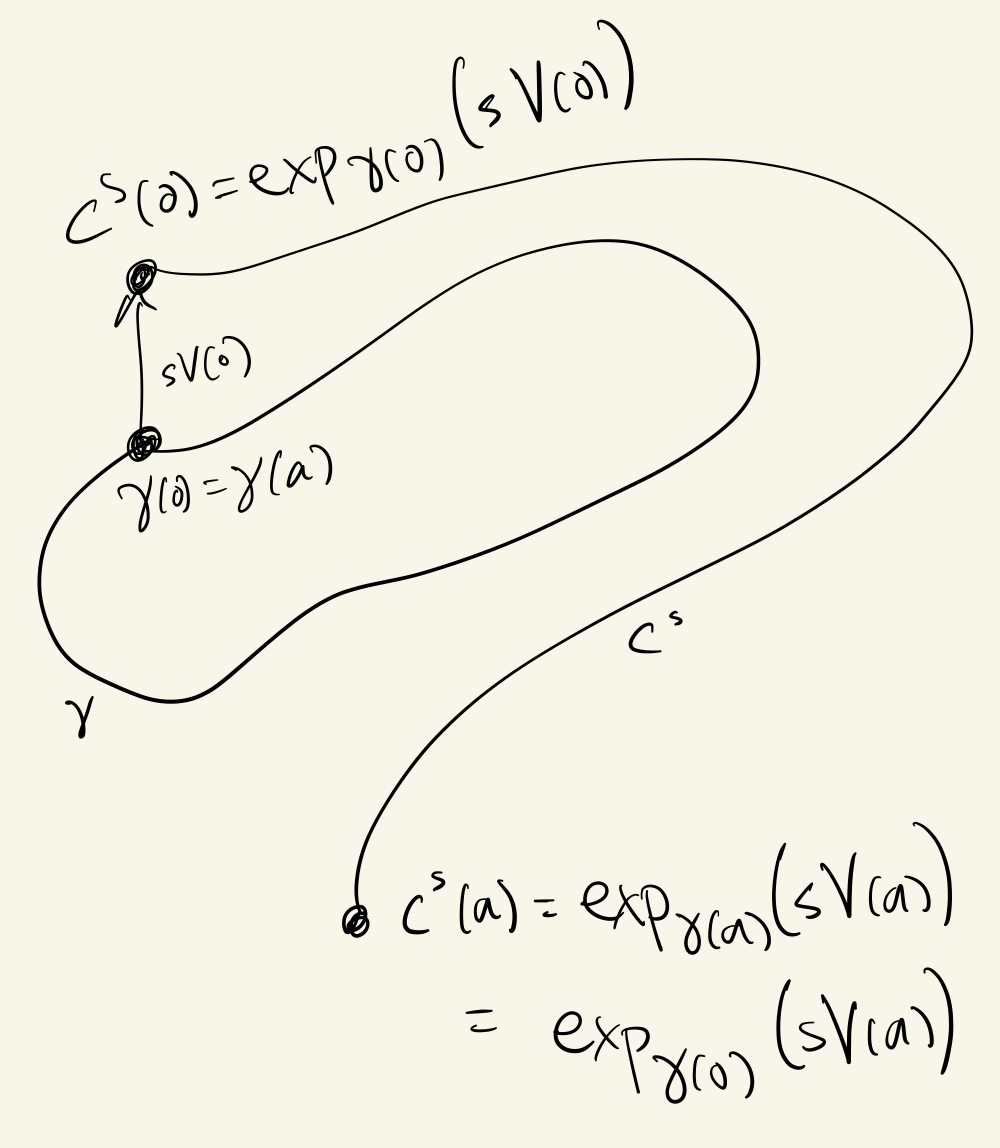
\includegraphics[width=0.5\textwidth]{figures/free-homotopy-variation}
\end{figure}
Fica claro que se $V(0)=V(a)$ as curvas $c^s$ são fechadas para toda $s$. Então
a condição que precisamos é que \[P^\gamma_{0,a}V(0)=V(a)\] onde $P$ é o
transporte paralelo. Dito de outra forma, basta ver que $P$ tem um ponto
fixo---além de $\gamma'(0)=\gamma'(a)$, que já é um ponto fixo. Esse argumento é
uma imitação da prova do teorema de Weinstein: como $P$ preserva orientação, o
determinante dele deve ser positivo, ou seja, o produto dos seus autovalores
deve ser positivo. Restringindo-nos ao subespaço $\gamma'(0)^\perp$, que tem
dimensão ímpar, concluímos que para que o produto dos autovalores de $P$ seja
positivo, deve ter pelo menos um que seja $1$.
\end{proof}

\section{Lista 7}
\label{section-lista-7}

\begin{exercise}
\label{exercise-minimizing-implies-no-conjugate-points}
Seja $\gamma:[0,a]\to M$ uma geodésica em uma variedade Riemanniana $M$.

 Prove que se $\gamma$ é minimizante, então $\gamma$ não possui pontos
 conjugados em  $(0,a)$. Encontre um exemplo de geodésica $\gamma:[0,a] \to M$ 
sem pontos conjugados que não é minimizante.
\end{exercise}

\section{Lista 8}
\label{section-lista-8}

\begin{exercise}
\label{exercise-l8-1}
Prop. 2.12 do capítulo XIII, \cite{doc}. Seja $p \in M$. 
Suponha exista um ponto $q \in C_m(p)$ que realiza a distância de $p$ a 
$C_m(p)$. Então:
\begin{enumerate}
\item ou existe uma geodésica 
minimizante $\gamma$ de $p$ a $q$ ao longo da qual $q$ é 
conjugado a $p$,
\item ou existem exatamente duas geodésicas 
minimizantes $\gamma$ e $\sigma$ de $p$ a $q$; além disto,
$\gamma'(\ell)=-\sigma'(\ell)$, 
$\ell=d(p,q)$. 
\end{enumerate}
\end{exercise}

\begin{proof}
No final da secção 1 do Capítulo XIII está especificado que as variedades que se
consideram no capítulo são completas. Portanto podemos supor que existe
uma geodésica minimizante $\gamma$ ligando $p$ e $q$.

Então podemos aplicar a Proposição \ref{proposition-cut-point-characterization}:
 um ponto $q$ é o cut point de $p$ ao longo de uma 
geodésica minimizante $\gamma$ se e somente se
alguma das seguintes condições é verdadeira: 
(a) $q$ é o primeiro ponto conjugado a $p$ ao longo de $\gamma$, ou 
(b) existem duas geodésicas minimizantes ligando $p$ e $q$.

Se (a) é verdadeira, terminamos. Se (b) é verdadeira, temos que existe outra
geodésica minimizante $\sigma$ ligando $p$ e $q$.

{\bf Intento pessoal (não funcionou):}  considere a variação por geodésicas 
$$
f(s,t):=\operatorname{exp}_{\gamma(t)}
(s\operatorname{exp}_{\gamma(t)}^{-1}\sigma(t))
$$
cujo campo de Jacobi 
$$
J(t)=d_{t\text{exp}_{\gamma(t)}^{-1}\sigma(t)}
\text{exp}_p(\text{exp}_{\gamma(t)}^{-1}\sigma(t))
$$
se anula em $t=0,1$. Pensei que esse campo de Jacobi estava bem definido pelo 
Corolário 2.8, Cap. XIII (Lema 
\ref{lemma-outside-cut-locus-exists-minimizing-geodesic}), que assegura
 que $\text{exp}_p$ é injetiva fora do cut locus de $p$. Porém, precisaria
 que a exponencial ao longo de $\gamma$,
 $\text{exp}_{\gamma(t)}$, for injetiva fora do cut locus de $p$. 
Essa condição seria garantida se $d(p,q)=i(M)$, ou seja, se a exponencial
 $\text{exp}_{p'}$ for injetiva na bola de raio $d(p,q)$ para qualquer 
$p' \in M$. Em conclusão: minha variação não está bem definida. 
(Se estivesse, com
isso terminaria o exercício, pois obtemos que o único caso em que $p$ não é
conjugado a $q$ é se $\gamma'(\ell)=-\sigma'(\ell)$, i.e. se o campo de Jacobi 
associado à variação é nulo.) 

\bigskip

A variação certa é produzida no \cite{doc} supondo que 
$\gamma'(\ell)\neq -\sigma'(\ell)$; isso implica que existe um vetor
 $V \in T_q M$ tal que 
$\left<\gamma'(\ell),V\right>< 0$ e $\left<\sigma'(\ell),V\right>< 0$.

Uma maneria simples de conferir a existência desse vetor $V$ é olhando para o 
plano gerado por $\gamma'(\ell)$ e $\sigma'(\ell)$ (usando que são linearmente
independentes). O conjunto de vetores $V$ nesse plano satisfazendo 
$\left<\gamma'(\ell),V\right><0$ é um semiespaço, e o mesmo acontece com 
 os vetores satisfazendo $\left<\sigma'(\ell),V\right><0$. Esses dois semiespaços
devem ter interseção não vazia precisamente porque 
$\gamma'(\ell)\neq -\sigma'(\ell)$.

Agora usamos o fato de que $p$ e $q$ não são conjugados para 
achar uma vizinhança do vetor $\ell \gamma'(0)$ onde $\text{exp}_p$ é um
difeomorfismo e assim levantar alguma
curva $r$ que realize o vetor $V$ ao espaço tangente,
 digamos $v:(-\varepsilon,\varepsilon) \to T_q M$.

A variação então está dada por
$$
f(s,t):=\text{exp}_p\left(\frac{t}{\ell}v(s)\right)
$$
Podemos aplicar a primeira fórmula da variação, na qual: o termo com a
integral é zero porque $\gamma$ é uma geodésica; o termo da sumatoria é zero
porque trata-se de uma variação suave; e o primeiro termo dos extremos é zero
porque a variação fixa o ponto de partida. Obtemos que 
$$
E'(0)=\left<V,\gamma'(0)\right><0
$$
Note que Manfredo escreve a equação anterior usando o funcional de distância. 
Isso também é válido: de fato a primeira fórmula da variação pode ser 
deduzida de maneira análoga (feito em sala para variações próprias) 
 para o funcional de distância no caso de geodésicas parametrizadas por 
comprimento de arco (cf. Teo. 6.3 \cite{ler}).

O fato da derivada do funcional de comprimento ser negativa nos diz que para
valores perto de $s=0$ podemos achar curvas com menor comprimento. Mais
precisamente, existe um $s>0$ tal que $\ell(f(s,\cdot))<\ell(\gamma)$.

É claro que o mesmo procedimento genera uma variação $\tilde{f}$ de $\sigma$, e 
podemos supor que a mesma $s>0$ faz $\ell(\tilde{f}(s,\cdot))<\ell(\sigma)$.

Concluímos seguindo o argumento do Professor Manfredo: se 
$\ell(\gamma_s)=\ell(\sigma_s)$, então temos duas geodésicas com o mesmo
comprimento ligando $p$ e $\gamma_s(\ell)=\sigma_s(\ell)$; isso significa 
que existe um ponto $\tilde{t} \in (0,\ell]$ tal que $\gamma_s(\tilde{t})$ é
 o cut point de $p$. Porém, isso contradiz o fato de que $q$ realiza a 
distância entre $p$ e o seu cut locus.

Finalmente, se $\ell(\gamma_s)<\ell(\sigma_s)$, segue que o cut point de $p$
 ao longo de $\sigma_s$ está a distância menor do que $q$, que de novo contradiz
a nossa hipótese.
\end{proof}

\begin{exercise}
\label{exercise-l8-2}
Proposição 2.13, Cap. XIII \cite{doc}. Se a curvatura seccional $K$ de uma
variedade Riemanniana completa $M$ satisfaz
$$
0< K_{\operatorname{min}}\leq K\leq K_{\operatorname{max}},
$$
Então
\begin{enumerate}
\item $i(M) \geq \pi/\sqrt{K_{\operatorname{max}}}$, ou
\item existe uma geodésica fechada $\gamma$ em $M$, cujo comprimento é menor do 
que o de qualquer outra geodésica fechada em $M$, tal que
$$
i(M)=\frac{1}{2}\ell(\gamma)
$$
\end{enumerate}
\end{exercise}

\begin{proof}
Suponha que (1) não é verdadeiro. 

Note que pelo Teorema de Bonnet-Myers 
\ref{theorem-Bonnet-Myers}, $M$ é compacta e portanto $C_m(p)$ é compacto para
todo $p$. Isso nos permite achar dois pontos $p$ e $q$ cuja distância é o raio
de injetividade  $i(M)$.

Então podemos usar o exercício anterior para $p$ e $q$.  Primeiro vamos ver o
que acontece no caso da segunda possibilidade daquele exercício, i.e. que
existam exatamente duas geodésicas ligando $p$ e $q$, digamos $\gamma$ é
$\sigma$, tais que $\gamma'(\ell)=-\sigma'(\ell)$ onde $\ell=d(p,q)$.  Considere
$\gamma * \overline{\sigma}$, onde $*$ é a concatenação de curvas e 
$\overline{\sigma}$ é a curva $\sigma$ percorrida em sentido contrário. É claro
que $\gamma * \overline{\sigma}$ é uma geodésica fechada de comprimento $2
d(p,q)$. Note que por definição  $d(p,q)=\ell=i(M)$, como queríamos.

Essa geodésica fechada tem a distância mínima entre as geodésicas fechadas, já
que se tivéssemos alguma outra com distância menor, podemos pegar um ponto
qualquer nela e o seu cut point ficaria a distância exatamente a metade do
comprimento do laço (pois existem duas geodésicas que chegam nele: cada
metade do laço partindo em direções opostas do ponto inicial escolhido),
contradizendo o fato de que $i(M)=d(p,q)$.

Portanto, basta descartar o primeiro caso do exercício anterior. Para chegar a
 uma contradição, suponha que $p $ é conjugado a $q$, i.e. que existe um campo
 de Jacobi $J$ que se anula em $p$ e em $q$. Podemos usar o teorema de Rauch
\ref{theorem-Rauch} para comparar esse campo com $\tilde{J}$, 
um campo em $S^n_{K_{\text{max}}}$, a esfera de curvatura constante
 $K_{\text{max}}$. Como $K \leq  K_{\text{max}}$,
concluímos que $\tilde{J}$ deve se anular em $\ell=d(p,q)=i(M)$. Absurdo, pois
estamos supondo que (1) não é verdadeiro, i.e. que
 $i(M) < \pi/\sqrt{K_{\text{max}}}$.
\end{proof}

\begin{exercise}
\label{exercise-l8-3}
\cite{doc}, Capítulo XIII, Proposição 3.4. Se a curvatura seccional $K$ de uma
variedade Riemanniana $M^n$, compacta, orientável e de dimensão par, satisfaz 
$0<K \leq 1$, então $i(M) \geq \pi$.
\end{exercise}

\begin{proof}
Para obter uma contradição, suponha que existe um ponto $p \in M$ tal que
 $d(p, C_m(p))<\pi$. Como $M$ é compacta, sabemos que $C_m(p)$ é compacto e
portanto existe uma geodésica $\gamma$ ligando $p$ com $q \in C_m(p)$ e
realizando a distância $d(p,C_m(p))$.

Pelo teorema de Rauch, sabemos que qualquer geodésica não pode ter pontos
conjugados antes de alcançar comprimento $\pi$. Explicitamente, se $J$ é um
campo de Jacobi ao longo de alguma geodésica $\gamma$ tal que $J(0)=0$ e 
$J(\ell(\gamma))=0$, comparando com um campo $\tilde{J}$ em $S^n$ tal que
 $\tilde{J}(0)=0$, $|\tilde{J}'(0)|=|J'(0)|$ e 
$\left<J,\gamma'\right>=\left<\tilde{J},\tilde{\gamma}\right>$, concluímos que
 $|\tilde{J}|\leq |J|$ ao longo de $\gamma$. Como as geodésicas de $S^n$ não
 tem pontos conjugados antes de atingir comprimento $\pi$, concluímos que 
$J$ não pode se anular antes desse ponto.

Isso mostra que, como estamos supondo que $d(p,C_m(p))<\pi$, devemos estar no
caso (2) do Exercício \ref{exercise-l8-1}, i.e. existem exatamente duas
geodésicas $\gamma$ e $\sigma$ ligando $p$ e $q$, e
$\gamma'(\ell)=-\sigma'(\ell)$. Repetindo o procedimento do Exercício anterior
 \ref{exercise-l8-3}, podemos usar essas duas geodésicas para achar uma 
geodésica fechada de comprimento $2i(M)$, cujo comprimento é menor do que o
comprimento de qualquer outra geodésica fechada.

\begin{remark}
\label{remark-curvatura-positiva-implica-maior-que-constante-positiva}
Na prova do teorema de Synge \ref{theorem-Synge}, o Professor
Manfredo afirma que ``Como $M$ é compacta e tem curvatura positiva, $K\geq
\delta>0$"; que não me parece imediato, pois a curvatura seccional não é uma
função definida em $M$. Porém, não preciso mostrar isso para garantir a
existência do loop geodésico (via o exercício anterior); apenas é necessário 
que $M$ seja compacta para garantir a existência do ponto $q$.
\end{remark}

\medskip

Para concluir seguimos a prova de \cite{doc}. Vamos a usar o exercício 6 da
lista 6, (cf. \ref{exercise-free-homotopy-variation}), onde mostrei que, nestas condições, i.e.
$M$ de dimensão par, completa, orientável e com curvatura seccional positiva,
existem curvas livremente homotópicas a qualquer geodésica fechada $\gamma$, que
possuem comprimento menor que $\ell(\gamma)$. Lembre que essas curvas foram
construídas mediante a função exponencial aplicada a um campo paralelo ao longo
de $\gamma$, de forma que são curvas suaves; vou usar esse fato depois.

A ideia é chegar numa contradição mostrando que existe uma terceira geodésica
ligando $p$ e $q$. Essa geodésica se obtém como o limite de uma sequência de
geodésicas associada à variação dada pelo Exercício 6 da Lista 6.

Seja $c_s$ uma das curvas da variação com comprimento estritamente
menor do que $\ell(\gamma)$. Pegue o ponto inicial $c_s(0):=\tilde{p}_s$ e o 
ponto $\tilde{q}_s$ em $c_s$ tal que $d(\tilde{p}_s,\tilde{q}_s)$ é máxima ao 
longo de $c_s$. Existe uma geodésica $\tilde{\gamma}_s$ que liga 
$\tilde{p}_s$ e $\tilde{q}_s$.

A seguir mostrarei que tomando limite quando $s \to 0$, obteremos uma terceira
geodésica minimizante $\tilde{\gamma}_0$ que liga $p$ e $q$, que não é possível
de novo pelo Exercício \ref{exercise-l8-1}.

De fato, podemos dar explicitamente $\tilde{\gamma}_0$ como sendo $exp_q(tw)$
onde $w$ é o vetor limite das velocidades iniciais de cada $\tilde{\gamma}_s$,
supondo que elas são de tamanho 1 para assegurar a existência do limite por
compacidade do fibrado tangente unitário. Note que a geodésica obtida minimiza a
distância entre $p$ e $q$: a geodésica liga $p$ com  $q$ porque, por um lado, o
limite dos pontos iniciais é $p$ por definição, e, por outro lado, porque os
pontos finais são os pontos que maximizam a distância dentro de cada geodésica.
A geodésica limite é minimizante por continuidade da função distância.

Como cada curva $c_s$ é diferenciável, temos um vetor tangente a ela em cada
ponto $\tilde{q}_s$. Como $\tilde{\gamma}$ é minimizante, quando aplicamos a
fórmula da primeira variação,vemos que $\tilde{\gamma}'_s$ é ortogonal a
$c_s'(\tilde{q}_s)$. Como o a métrica é contínua, concluímos que
$\tilde{\gamma}_0'(q) \perp \gamma'(q)$.
\end{proof}

\begin{exercise}
\label{exercise-l8-11}
Seja $M$ uma variedade Riemanniana completa, de curvatura seccional não
negativa. Sejam $\gamma,\sigma:[0,\infty) \to M$ geodésicas tais que
$\gamma(0)=\sigma(0)$. Se $\gamma$ é um raio e
$\angle(\gamma'(0),\sigma'(0))<\frac{1}{2}\pi$, então $\lim_{t \to \infty}
\rho(\sigma(0),\sigma(t))=\infty$ (i.e. $\sigma$ vai para o infinito).
\end{exercise}

\begin{proof}[Meu intento de prova]
Seja $t \in \mathbb{R}$. Considere uma geodésica minimizante $\tau_t$ ligando
$\gamma(t)$ com $\sigma(t)$. Defina o angulo 
$\beta_t:=\angle(-\gamma'(t),\tau'_t(0))$ e o número $s_t$ como sendo o tempo em que
$\tau_t$ chega em $\sigma$, i.e. $\tau_t(s_t)=\sigma(t)$. Ver Figura
\ref{figure-toponogov-exercise}.

Como $0 \leq  K$, podemos comparar a ``hinge'',
i.e. a informação do angulo e vetores incidentes no ponto $\gamma(t)$, 
$(-\gamma'(t),\tau_t'(0),\beta)$ com uma hinge no espaço
euclidiano. Obtemos que 
$$
\rho_{\mathbb{R}^n}(\tilde{\gamma}(0),\tilde{\tau}_t(s_t))\leq
\rho(\gamma(0),\tau_t(s_t))=\rho(\sigma(0),\sigma(t))
$$
\begin{figure}[H]
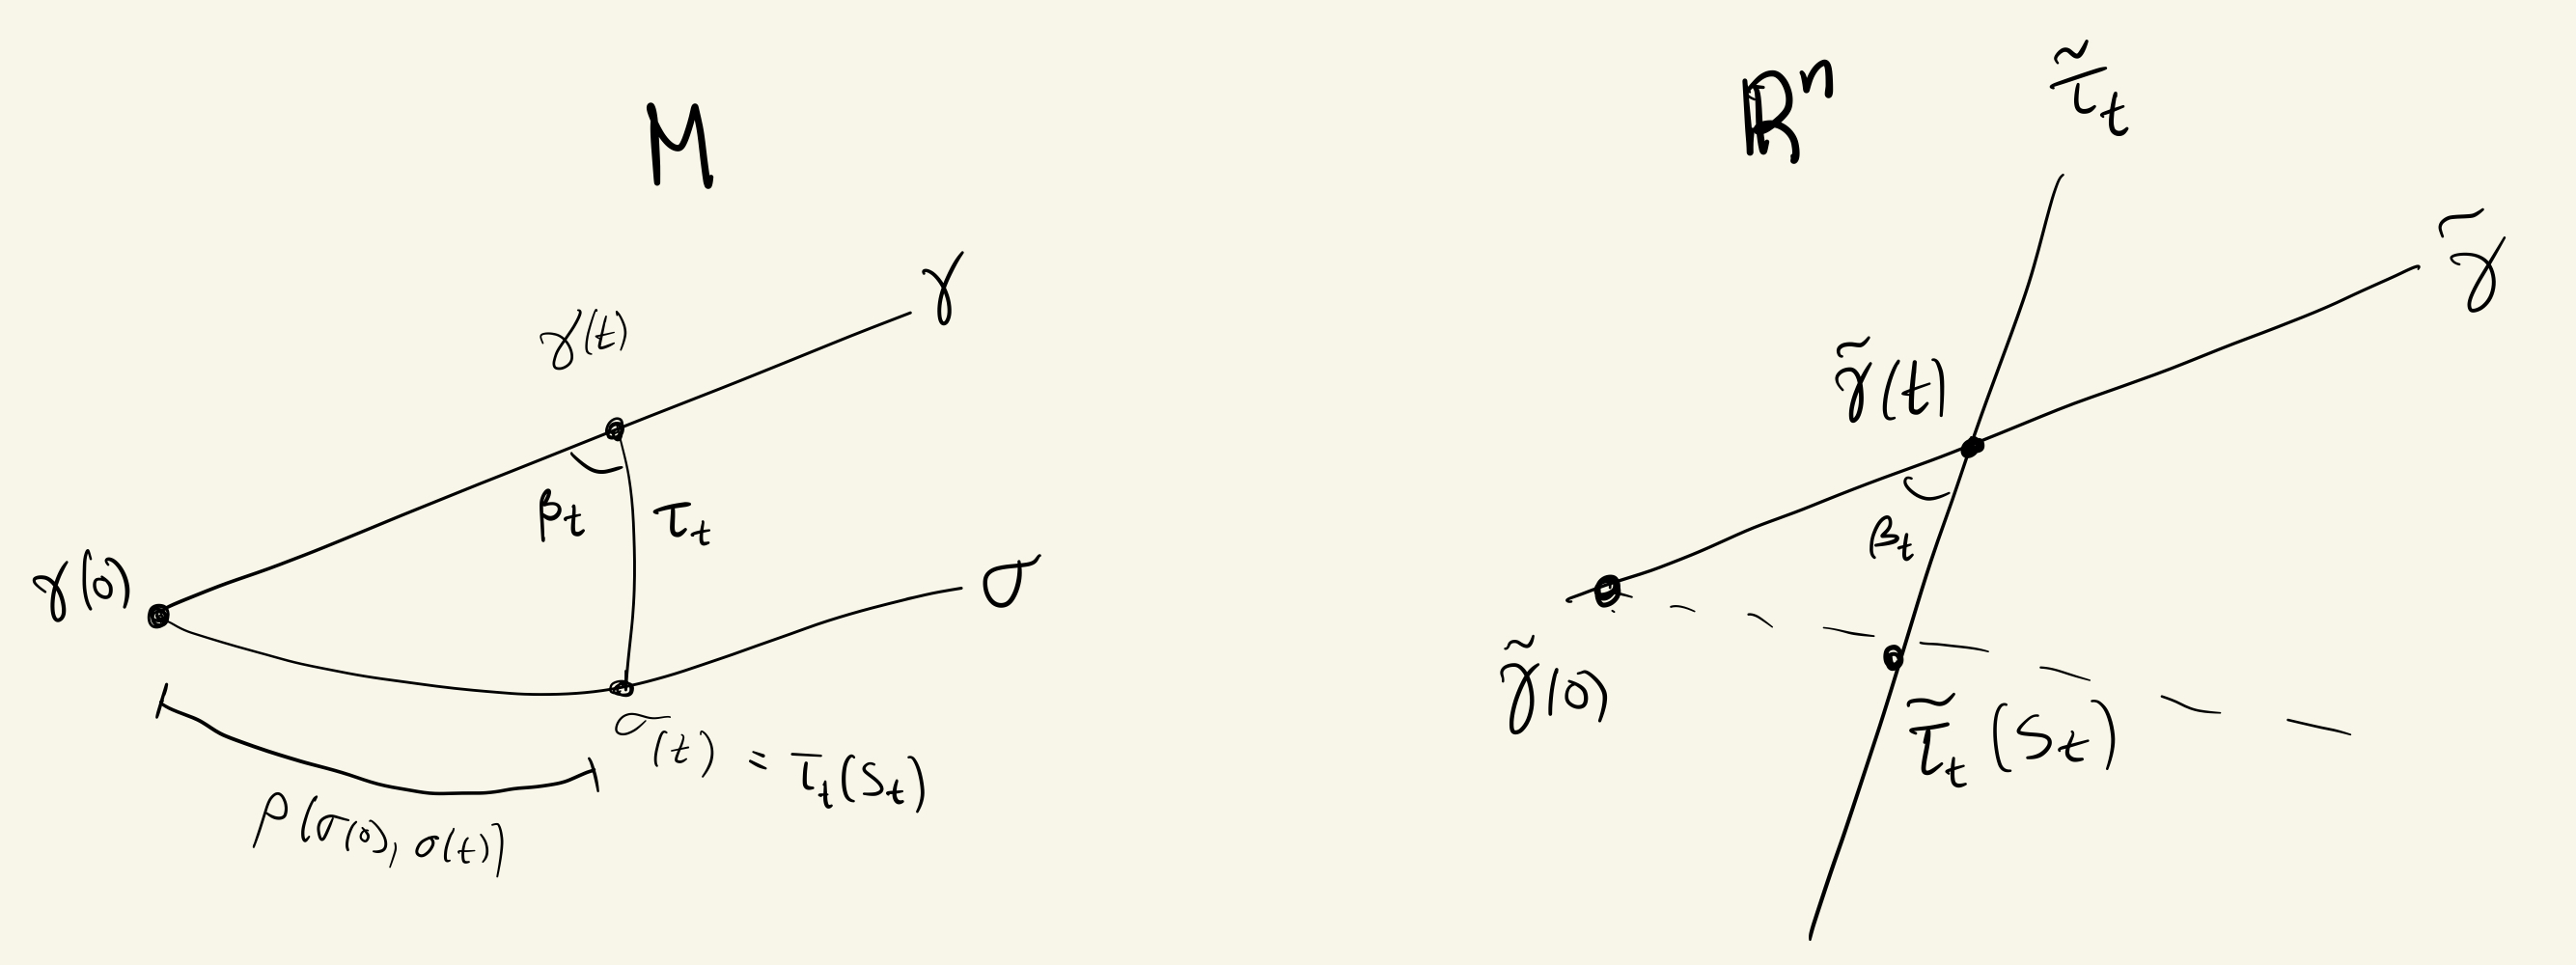
\includegraphics[width=1\textwidth]{figures/toponogov-exercise}
\caption{}
\label{figure-toponogov-exercise}
\end{figure}
Podemos calcular a distância
$\rho_{\mathbb{R}^n}(\tilde{\gamma}(0),\tilde{\tau}_t(s_t))$ usando a lei de
cosenos euclidiana desde que conheçamos $\beta_t$ e $\ell(\tau_t)$:
$$
\rho_{\mathbb{R}^n}(\tilde{\gamma}(0),\tilde{\tau}_t(s_t))^2=
t^2+\ell(\tau_t)^2-2t\ell(\tau_t)\cos \beta_t
$$
Para calcular $\ell(\tau_t)$ podemos usar o Teorema de Toponogov de novo, dessa
vez comparando a hinge $(\gamma'(0), \sigma'(0),\alpha)$ com uma correspondente
no espaço euclidiano:
\begin{figure}[H]
\centering
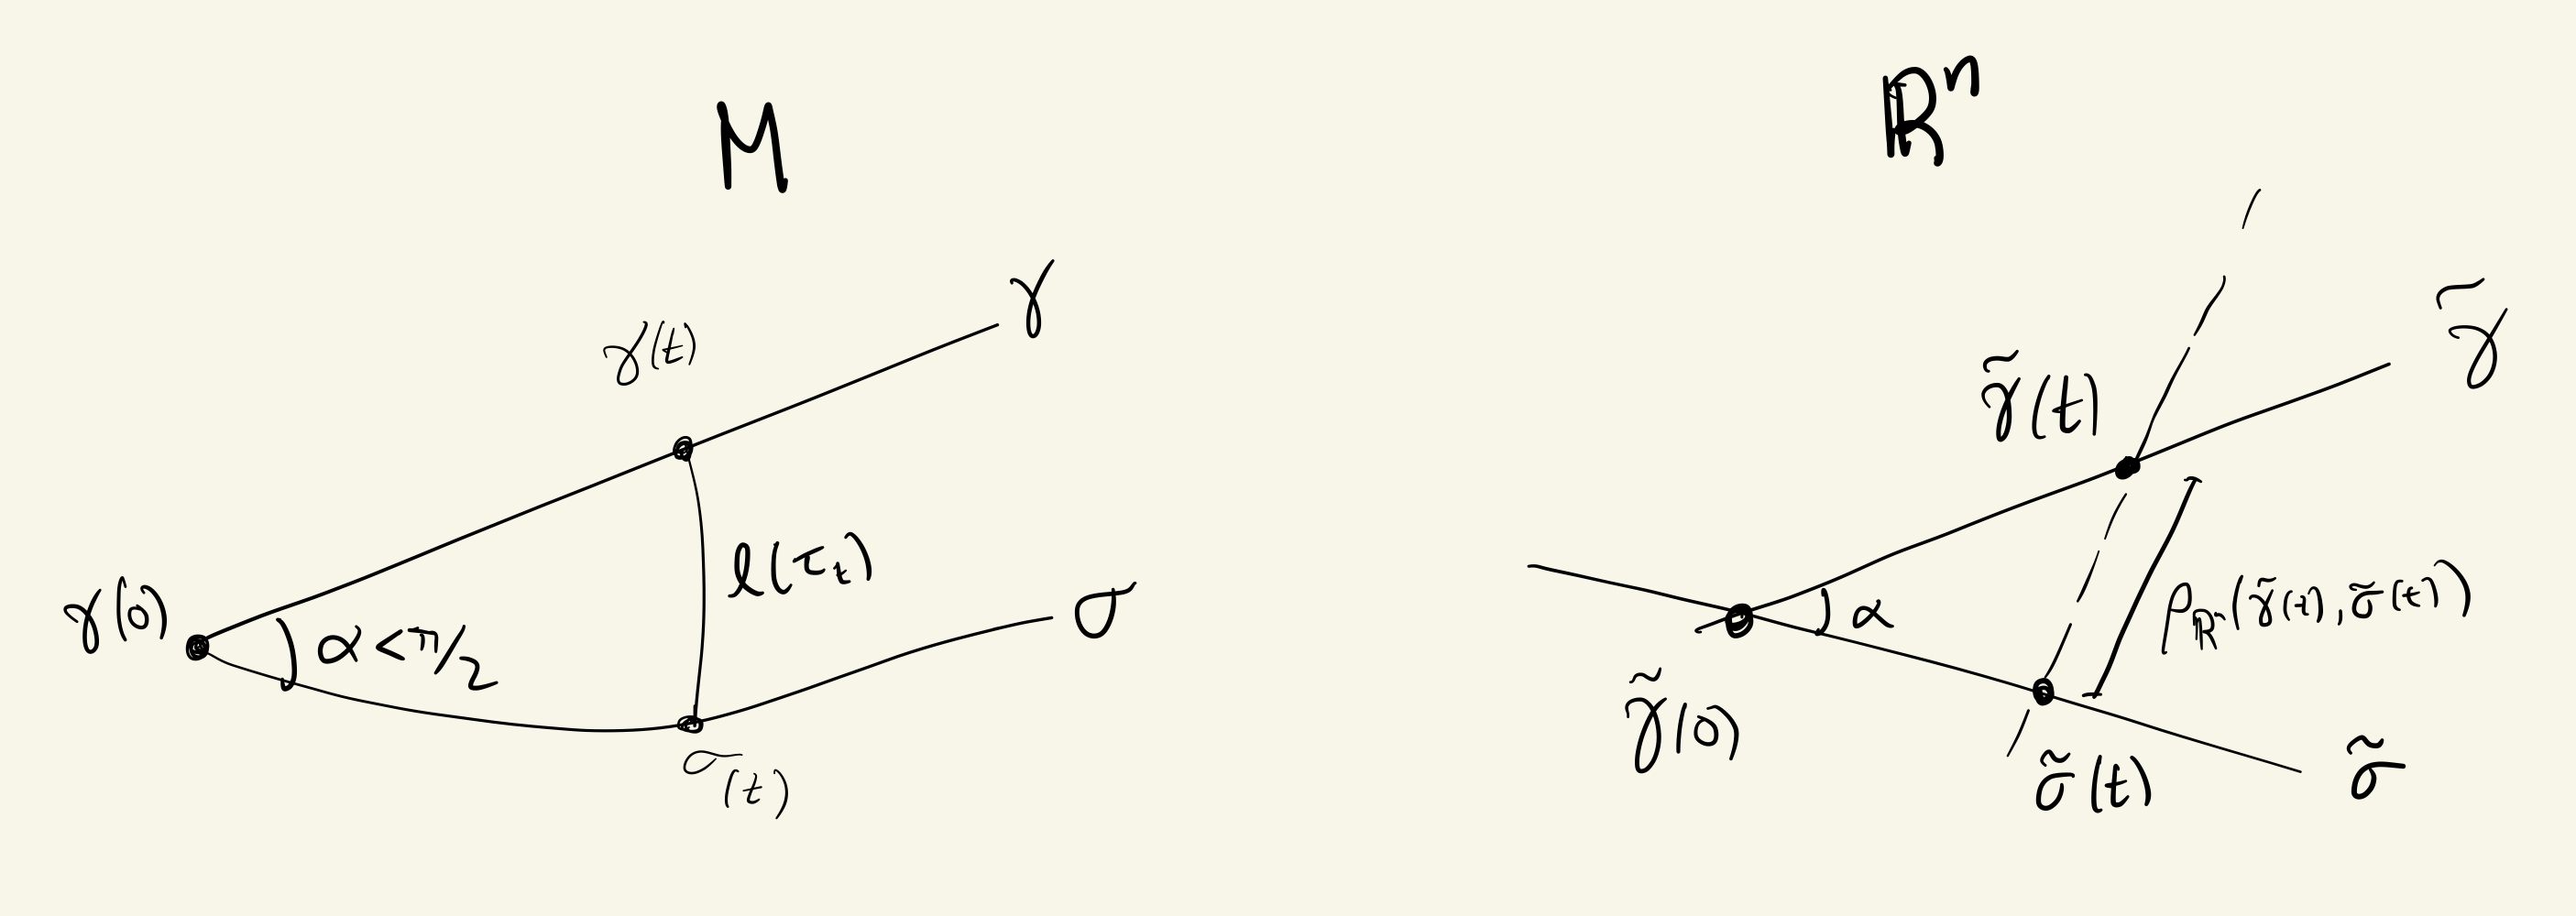
\includegraphics[width=1\textwidth]{figures/toponogov-exercise2}
\label{figure-toponogov-exercise2}
\end{figure}
Obtemos que
$$
\rho_{\mathbb{R}^n}(\tilde{\gamma}(t),\tilde{\sigma}(t))\leq \ell(\tau_t)
$$
Como $\alpha$ é constante conforme $t$ muda, podemos fixar $\tilde{\gamma}$ e
$\tilde{\sigma}$ para fazer a nossa comparação. Conforme  $t$ avança, nos
movemos a velocidade constante ao longo de $\tilde{\gamma}$ en direção ao
infinito, e embora não sabemos se a distância $\rho(\sigma(0),\sigma(t))$ cresse
 ou diminue, a distância do nosso interesse 
$\rho_{\mathbb{R}^n}(\tilde{\gamma}(t),\tilde{\sigma}(t))$
vai sempre crescendo, e concluimos que diverge ao infinito.

Portanto o problema acaba se conseguimos achar uma cota inferior positiva para
$\beta_t$. Parece que isso é equivalente a provar que a distância entre
$\gamma$ e $\sigma$ está acotada inferiormente por uma constante positiva…

A lei de cosenos do lado Euclideano nos diz que
$$
\rho_{\mathbb{R}^n}(\tilde{\gamma}(t),\tilde{\sigma}(t))^2=
t^2+|\tilde{\sigma}(t)|^2-2t |\tilde{\sigma}(t)|\cos \alpha
\leq t^2+|\tilde{\sigma}(t)|^2-2t |\tilde{\sigma}(t)|
$$
Supondo que $\tilde{\gamma}(0)=\tilde{\sigma}(0)=0 \in \mathbb{R}^n$. 
Parece que para medir essa distância deveríamos conhecer
$|\tilde{\sigma}(t)|=\rho(\sigma(0),\sigma(t))$...
 o que parece levar o problema de volta ao
problema inicial.
\end{proof}

\begin{proof}[Prova de \cite{Cheeger-Ebin}]
Por desigualdade triangular, para quaisquer $t,s \in \mathbb{R}$,
$$
\rho(\sigma(t),\sigma(0)) \geq
\rho(\gamma(s),\sigma(t))-\rho(\gamma(s),\gamma(0)).
$$
Como o lado esquerdo não depende de $s$, vemos que basta tomar o limite quando 
$s\to \infty$ e mostrar que esse limite está inferiormente limitado por um
número que depende linearmente de $t$, i.e. $t \cos\alpha$.

Considere uma geodésica minimizante $\tau_{s,t}$ ligando $\gamma(s)$ e
$\sigma(t)$. Podemos usar o teorema de Toponogov \ref{theorem-Toponogov-angle}
na versão de ângulos (que está enunciada em \cite{Cheeger-Ebin}) já que duas das
geodésicas no triângulo $\gamma(0),\gamma(s),\sigma(t)$ são minimizantes por
hipótese. Como a cota inferior da curvatura é 0 não temos problemas com o
comprimento de $\sigma$.

Obtemos que existe um triângulo Euclidiano com lados do mesmo comprimento tal
que os ângulos correspondentes são menores o iguais que os ângulos com que
começamos.

Denote $A:=\rho(\gamma(0),\gamma(s))=s$, $B:=\ell(\sigma(t))=t$ e
 $C:=\rho(\gamma(s),\sigma(t))=\ell(\tau_{s,t})$.
Nosso objetivo é limitar inferiormente $C-A$ conforme  $s \to \infty$.
 Aplicamos a lei de cosenos no lado Euclidiano para obter
\begin{align*}
C^2&=A^2+B^2-2AB\cos\tilde{\alpha}\\
\implies C^2-A^2&=B^2-2AB\cos\tilde{\alpha}\\
\implies C-A&=\frac{B^2-2AB\cos\tilde{\alpha}}{C+A}
\end{align*}
Onde só $A=s$ e $C$ dependem de $s$. O comportamento assintótico desse quociente
quando $s \to \infty$ é claro geometricamente: como $A$ e $C$ são dois lados de
um triângulo, eles crescem proporcionadamente. Formalmente, como $C \leq A+B$,
obtemos $C+A \leq 2A+B$. Daí
\begin{align*}
\frac{1}{C+A}&\geq \frac{1}{2A+B}\\
\implies \frac{B^2-2AB\cos \tilde{\alpha}}{C+A}&\geq
 \frac{B^2-2AB \cos \tilde{\alpha}}{2A+B}
=\frac{A}{A}\frac{B^2/A-2B\cos \tilde{\alpha}}{2+B/A}
\end{align*}
que (a menos de analizar o que acontece se o numerador é negativo…)
 converge a $B\cos \tilde{\alpha}$ conforme $s \to \infty$.
 Concluímos que $C-A$ deve
convergir a $-t\cos\tilde{\alpha}\leq-t\cos\alpha$. Tirando o signo obtemos a
desigualdade desejada.
\end{proof}
